\RequirePackage{fix-cm} 
\documentclass[smallextended]{llncs}
\usepackage[english]{babel}  
\usepackage{latexsym}
\usepackage{amsmath,amssymb}
\usepackage[dvips]{graphicx,psfrag}
\graphicspath{{figures/}}
\DeclareGraphicsExtensions{.eps}
\usepackage{color}
\usepackage{url}
\usepackage{booktabs}
\usepackage{todonotes}

\include{shorthand} % put your own shorthand declarations in this document
\newcommand{\vphi}{{\boldsymbol{\phi}}}
\renewcommand{\vec}[1]{\mathbf{#1}}
\newcommand{\phiproc}{$\phi_1$}
\newcommand{\phistartTime}{$\phi_2$}
\newcommand{\phiendTime}{$\phi_3$}
\newcommand{\phimacFree}{$\phi_4$}
\newcommand{\phimakespan}{$\phi_5$}
\newcommand{\phiwrmJob}{$\phi_6$}
\newcommand{\phiwrmMWR}{$\phi_7$}
\newcommand{\phislots}{$\phi_{8}$}
\newcommand{\phislotsTotal}{$\phi_{9}$}
\newcommand{\phislotsTotalperOp}{$\phi_{10}$}
\newcommand{\phiwait}{$\phi_{11}$}
\newcommand{\phislotCreated}{$\phi_{12}$}
\newcommand{\phitotProc}{$\phi_{13}$}
\newcommand{\PREF}[2]{PREF$_{#2}^{#1}$}

\usepackage{paralist}
\usepackage{graphicx}
\usepackage{subfig}
\usepackage{amssymb}
\usepackage{amsmath}
\usepackage[capitalise]{cleveref}

\newcommand{\shortcite}[1]{\cite{#1}}


\begin{document}
\title{Generating Training Data for Learning Linear \\ Composite Dispatching Rules for Scheduling}
\author{Helga Ingimundard\'ottir and Thomas Philip R\'unarsson}
\institute{{School of Engineering and Natural Sciences, University of Iceland}\\
\email{hei2@hi.is} and \email{tpr@hi.is}}

\maketitle
\begin{abstract}
A supervised learning approach to generating composite linear priority dispatching rules for scheduling is studied. In particular we investigate a number of strategies for generating training data for learning a linear dispatching rule using preference learning. The results show that generating training data set from optimal solutions only is not as effective as when suboptimal solutions are added to the set. Furthermore, different strategies for creating preference pairs is investigated as well as suboptimal solution trajectories. The different strategies are investigated on 2000 randomly generated problem instances using two different problems generator settings.
\end{abstract}

\noindent When applying learning algorithms, the training set is of paramount importance. Training set should have sufficient knowledge of the problem at hand. This is done by the use of features, which are supposed to capture the essential measures of a problem's state. For this purpose, the job-shop scheduling problem (JSP) is used as a case study to illustrate a methodology for generating a meaningful training data, which can be successfully learned. 

JSP deals with the allocation of tasks of competing resources where the goal is to minimise a schedule's maximum completion time, i.e., the makespan denoted $C_{\max}$. In order to find good solutions, heuristics are commonly applied in research, such as the simple priority based dispatching rules (SDR) from \cite{Panwalkar77}. Composites of such simple rules can perform significantly better \cite{Jayamohan04}. 
As a consequence a linear composite of dispatching rules (LCDR) was presented  in \shortcite{InRu11a}. The goal there was to learn a set of weights, $\vec{w}$, via logistic regression such that 
\begin{equation}\label{eq:jssp:linweights}
h(\vec{x}_j)=\big<{\vec{w}}\cdot{\vphi(\vec{x}_j)}\big>,
\end{equation}
yields the preference estimate for dispatching job $j$ that corresponds to post-decision state $\vec{x}_j$, where $\vphi(\vec{x}_j)$ denotes its feature mapping. The job dispatched is the following, 
\begin{equation}\label{eq:jstar}
j^* = \arg\max_j\left\{h(\vec{x}_j)\right\}. 
\end{equation}
The approach was to use supervised learning, to determine which feature states are preferable to others. 
The training data was created from optimal solutions of randomly generated problem instances. 

An alternative would be minimising the expected $C_{\max}$ directly using a brute force search such as CMA-ES \cite{Hansen01}. Preliminary experiments were conducted in \shortcite{InRu14a}, which showed that optimising the weights in \cref{eq:jssp:linweights} via evolutionary search actually resulted in a better LCDR than the previous approach. The nature of the CMA-ES is to explore suboptimal routes until it converges to an optimal one. Implying that the previous approach of restricting the training data only to \emph{one} optimal route may not produce a sufficiently rich training set. That is, the training set should incorporate a more complete knowledge on \emph{all} possible preferences, i.e., make also the distinction between suboptimal and sub-suboptimal features, etc.  This would require a Pareto ranking of preferences which can be used to make the distinction to which feature sets are equivalent, better or worse -- and to what degree, e.g. by giving a weight to the preference. This would result in a very large training set, which of course could be re-sampled in order to make it computationally feasible to learn. In this study we will investigate a number of different ranking strategies for creating preference pairs.

Alternatively, training data could be generated using suboptimal solution trajectories. For instance \cite{Siggi05} used decision trees to `rediscover' largest processing time (LPT),  a single priority based dispatching rule, by 
using LPT to create its training data. The limitations of using heuristics to label the training data is that the learning algorithm will mimic the original heuristic (both when it works poorly and well on the problem instances) and does not consider the real optimum. In order to learn heuristics that can outperform existing heuristics, then the training data needs to be correctly labelled. This drawback is confronted in \cite{Malik08,Russell09,Siggi10} by using an optimal scheduler, computed off-line. In this study, we will both follow optimal and suboptimal solution trajectories, but for each partial solution the preference pair will be labelled correctly by solving the partial solution to optimality using a commercial software package \cite{gurobi}. 
For this study most work remaining (MWR), a promising SDR for the given data distributions \cite{InRu12}, and the CMA-ES optimised LCDRs from \cite{InRu14a} will be deemed worthwhile for generating suboptimal trajectories.

To summarise, the study considers two main aspects of the generation of training data: 
\begin{inparaenum}[\itshape a\upshape)] 
\item how preference pair are added at each decision stage, and
\item which solution trajectorie(s) should be sampled. That is, optimal, random, or suboptimal ones, based on a good 
heuristic, etc.
\end{inparaenum}

The outline of the paper is as follows, first we illustrate how JSP can be seen as a decision tree where the depth of the tree corresponds 
total number of job-dispatches needed to form a complete schedule. The feature space is also introduced and how  optimal dispatches and suboptimal dispatches are labelled at each node in the tree. This is followed by detailing the strategies investigated in this study by selecting preference pairs ranking and sampling solution trajectories. The authors then perform an extensive study comparing these strategies. Finally, this paper concludes with discussions and summary of main results.

\section{Problem Space}
In this study synthetic JSP  data instances are considered with the problem size $n\times m$, where $n$ and $m$ denotes  number of jobs and machines, respectively. 
Problem instances are generated stochastically by fixing the number of jobs and machines and processing time are i.i.d. and sampled from a discrete uniform distribution from the interval $I=[u_1,u_2]$, i.e., $p\sim \mathcal{U}(u_1,u_2)$.
Two different processing times distributions are explored, namely 
$\mathcal{P}_{j.rnd}$ where $I=[1,99]$ and $\mathcal{P}_{j.rndn}$ where $I=[45,55]$, referred to as random and random-narrow, respectively.
The machine order is a random permutation of all of the machines in the job-shop. 

For each data distribution $N_{\text{train}}$  and $N_{\text{test}}$ problem instances were generated for training and testing, respectively. Values for $N$ are given in \cref{tbl:data:sim}. Note, that difficult problem instances are not filtered out beforehand, such as the approach in \cite{Whitley}. 

\begin{table}[t]\centering
\caption{Problem space distributions, $\mathcal{P}$. }\label{tbl:data:sim}
{\renewcommand{\arraystretch}{1.2}\footnotesize
\begin{tabular}{lcccl}\toprule
name&size ($n\times m$)& $N_{\text{train}}$&$N_{\text{test}}$  & note 
\\ \midrule
%\multirow{4}{*}{\begin{sideways}JSP\end{sideways}}
$\mathcal{P}_{j.rnd}$ & $6\times5$ & 500 & 500 & random \\
$\mathcal{P}_{j.rndn}$ & $6\times5$ & 500 & 500 & random-narrow \\
\bottomrule
\end{tabular}
}
\end{table}

\begin{table}[t]  \centering
  \caption{Feature space, $\mathcal{F}$.}
  \label{tbl:jssp:feat}
   { %\footnotesize
\centering
  \begin{tabular}{|ll|} %p{0.45\textwidth}|p{0.4\textwidth}|}
\hline
  $\vphi$ & Feature description \\
\hline
  \phiproc & job processing time \\
  \phistartTime & job start-time \\
  \phiendTime & job end-time\\
  \phimacFree & when machine is next free \\
  \phimakespan & current makespan \\   
  \phiwrmJob & total work remaining for job \\
  \phiwrmMWR & most work remaining for all jobs\\
  \phislots & total idle time for machine \\
  \phislotsTotal & total idle time for all machines \\
  \phislotsTotalperOp & \phislotsTotal\ weighted w.r.t. number of assigned tasks\\
  \phiwait & time job had to wait \\
  \phislotCreated & idle time created \\      
  \phitotProc & total processing time for job  \\
\hline
  \end{tabular}
}
 %Feature description for job $J_j$ on machine $M_a$ given current temporal schedule, where the set of jobs already dispatched are $J\subset\mathcal{J}$ on corresponding set of machines $\mathcal{M}_j\subset\mathcal{M}$

\end{table}

\section{JSP tree representation}\label{sec:gametree}
When building a complete JSP schedule $\ell=n\cdot m$ dispatches must be made consecutively. 
A job is placed at the earliest available time slot for its next machine, whilst still fulfilling constraints that each machine can handle, which is at most one job at each time, and jobs need to have finished their previous machines according to its machine order. 
Unfinished jobs, referred to as the ready-list denoted $\mathcal{R}$, are dispatched one at a time according to some heuristic. After each dispatch the schedule's current features are updated based on its resulting partial schedule. 
For each possible post-decision state the temporal features, $\mathcal{F}$, applied in this study are given in \cref{tbl:jssp:feat}, which are based on SDRs which are widespread in practice. For example if $\vec{w}$ is zero, save for $w_6=1$, then \cref{eq:jssp:linweights} gives $h(\vec{x}_j)>h(\vec{x}_i)$, 
$\forall i$ which are jobs with less work remaining than job $j$, namely \cref{eq:jstar} yields the job with the highest \phiwrmJob\ value, 
i.e., equivalent to dispatching rule most work remaining (MWR) 


\Cref{fig:jssp:gametree} illustrates how the first two dispatches could be executed for a $6\times 5$ JSP, with the machines, $a\in\{M_1,...,M_5\}$, on the vertical axis and the horizontal axis yields the current makespan, $C_{\max}$. The next possible dispatches are denoted as dashed boxes with the job index $j$ within and its length corresponding to processing time $p_{ja}$.
In the top layer one can see an empty schedule.
In the middle layer one of the possible dispatches from the layer above is fixed (depicted solid) and one can see the resulting 
schedule, i.e., what are the next possible dispatches given this new scenario? Finally, the bottom layer depicts all outcomes if job $J_3$ on machine $M_3$ would be dispatched. 
This sort of tree representation is similar 
to \emph{game trees} \cite{vonNeumann44} where the root node denotes the initial (i.e. empty) schedule and the leaf nodes 
denote the complete schedule, therefore the distance $k$ from an internal node to the root yields the number of 
operations already dispatched. Traversing from root to leaf node one can obtain a sequence of dispatches that yielded 
the resulting schedule, i.e., the sequence indicates in which order the tasks should be dispatched for that particular 
schedule. 

\begin{figure}[t!]
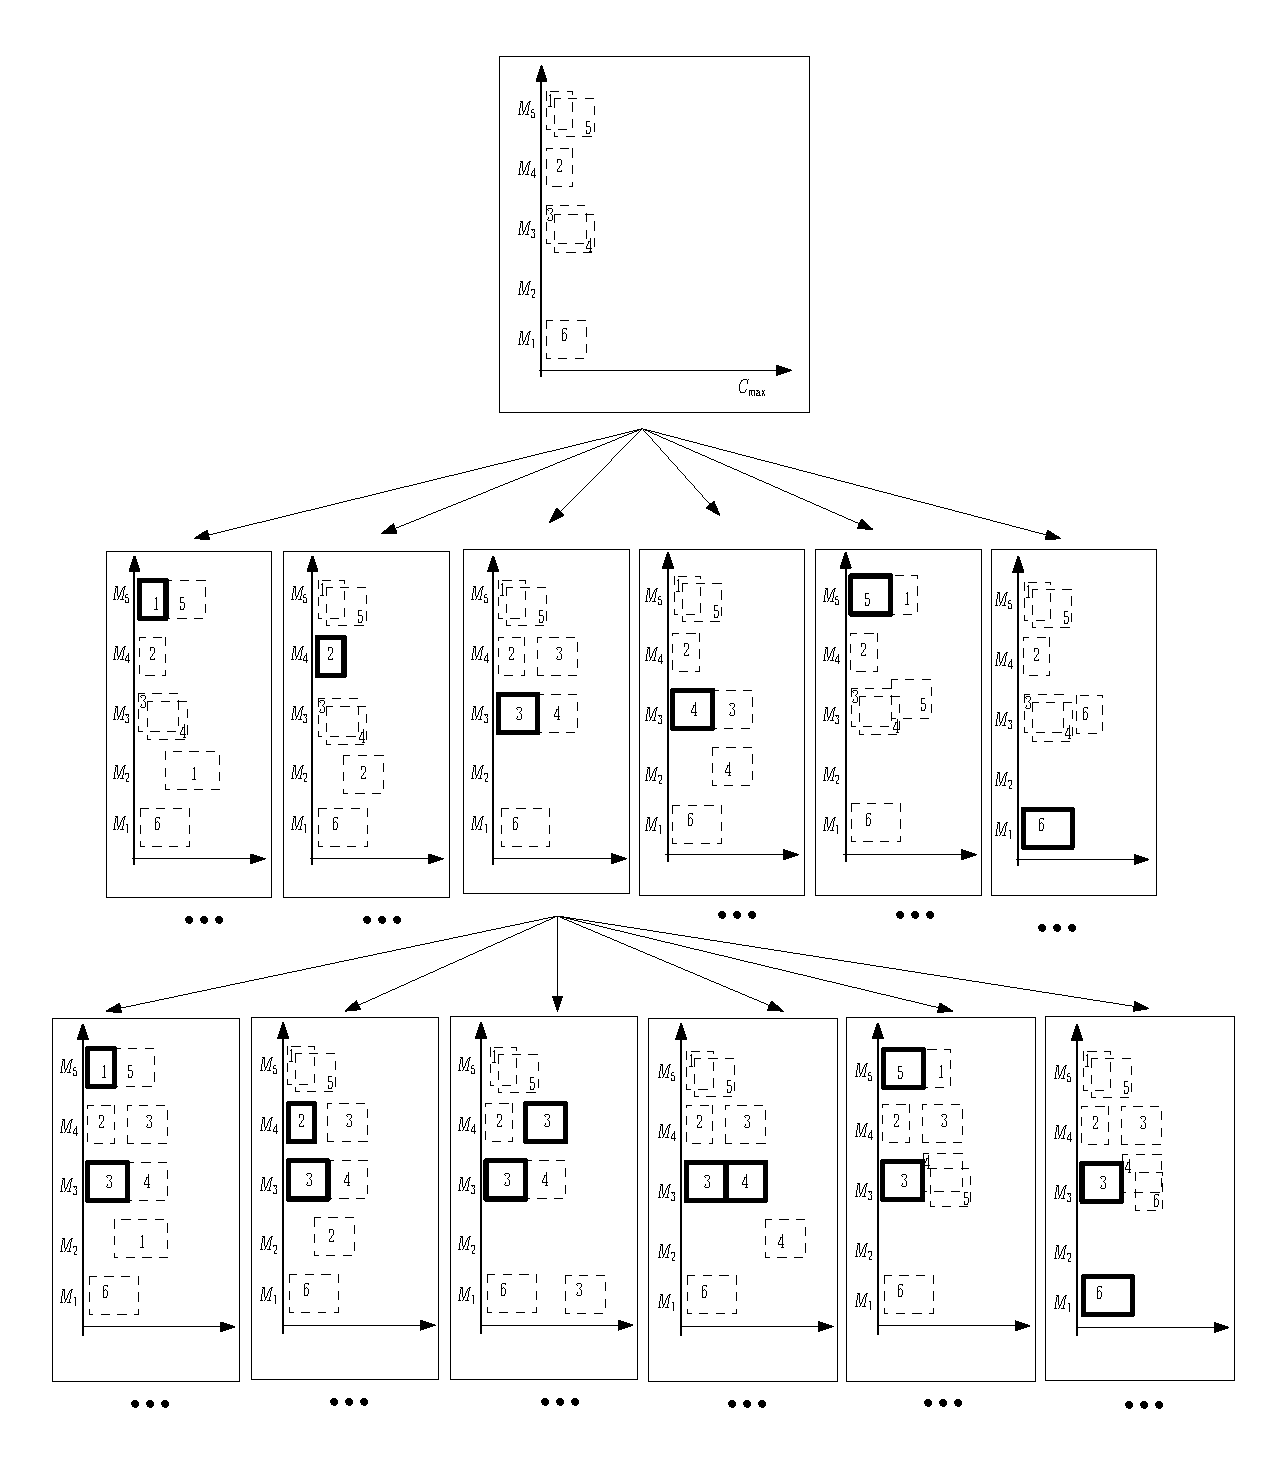
\includegraphics[width=\columnwidth]{figures/gametree}
\caption[Partial Game Tree for JSP]{Partial Tree for JSP for the first two dispatches. 
Executed dispatches are depicted solid, and all possible dispatches are dashed.}
\label{fig:jssp:gametree}
\end{figure}

However, one can easily see that this sequence of task assignments is by no means unique. Inspecting a partial 
schedule further along in the dispatching process such as in  \cref{fig:jssp:gametree} (top layer), then let's say 
$J_1$ 
would be dispatched next, and in the next iteration $J_2$. Now this sequence would yield the same schedule as if $J_2$ 
would have been dispatched first and then $J_1$ in the next iteration (since these are non-conflicting jobs). Which 
indicates that some of the nodes in the tree can merge. In the meantime the state of the schedules are different and 
thus their features, although they manage to merge with the same (partial) schedule at a later date.  % ATHUGASEMD 1 
%-- SEQ. REP NON-UNIQUE
In this particular instance one can not infer that choosing $J_1$ is better and $J_2$ is worse (or vice versa) since they can both yield the same solution.


Furthermore, in some cases there can be multiple optimal solutions to the same problem instance. Hence not only is the 
sequence representation `flawed' in the sense that slight permutations on the sequence are in fact equivalent w.r.t. 
the end-result, but varying permutations on the dispatching sequence (given the same partial initial sequence) can 
result in very different complete schedules but the same makespan, and thus same deviation from optimality, $\rho$ 
defined by \cref{eq:ratio}, which is the measure under consideration. Care must be taken in this case that neither 
resulting features are labelled as undesirable or suboptimal. Only the resulting features from a dispatch resulting in 
a suboptimal solution should be labelled undesirable. 

The creation of the tree for job-shop scheduling can be done recursively for all possible permutation of dispatches, 
in the manner described above, resulting in a full \mbox{$n$-ary} tree %(since $|\mathcal{R}|\leq n$)
of height $\ell=n\cdot m$. Such an exhaustive search would yield at the most $n^{\ell}$ leaf nodes (worst case scenario being that no sub-trees merge). Now, since the internal vertices (i.e. partial schedules) are only of interest to learn,\footnote{The root is the empty initial schedule and for the last dispatch there is only one option left to dispatch, so there is no preferred `choice' to learn.} the number of those can be at the most \mbox{${}^{n^{\ell}-1}/_{n-1}$} \cite{Rosen03}.
Even for small dimensions of $n$ and $m$ the number of internal vertices are quite substantial and thus 
computationally expensive to investigate them all. 
%Not to mention that this is done iteratively for all $N$ problem instances.

The optimum makespan is known for each problem instance. 
At each time step (i.e. layer of the tree) a number of feature pairs are created, they consist of the features 
$\vphi_o$ resulting from optimal dispatches $o\in\mathcal{O}^{(k)}$, versus features $\vphi_s$ resulting from 
suboptimal dispatches $s\in\mathcal{S}^{(k)}$ at time $k$. Note, 
$\mathcal{O}^{(k)}\cup\mathcal{S}^{(k)}=\mathcal{R}^{(k)}$ and $\mathcal{O}^{(k)}\cap\mathcal{S}^{(k)}=\emptyset$.
In particular, each job is compared against another job of the ready-list, $\mathcal{R}^{(k)}$, and if the makespan differs, i.e., $C_{\max}^{(s)} \gneq C_{\max}^{(o)}$, an optimal/suboptimal pair is created, however if the makespan would be unaltered the pair is omitted since they give the same optimal makespan. This way, only features from a dispatch resulting in a suboptimal solution is labelled undesirable.

The approach taken in this study is to verify analytically, at each time step, whether it can indeed \emph{somehow} yield an optimal schedule by manipulating the remainder of the sequence, yet maintaining the current temporal schedule fixed as its initial state. This also takes care of the scenario that having dispatched a job resulting in a different temporal makespan would have resulted in the same final makespan if another optimal dispatching sequence would have been chosen. That is to say the data generation takes into consideration when there are multiple optimal solutions to the same problem instance. 

\section{Selecting preference pairs}\label{sec:strategy}
At each dispatch iteration $k$ a number of preference pairs are created, which is then iterated over all $N_{\text{train}}$ problem instance created. A separate data set is deliberately created for each dispatch iterations, as the initial feeling is that DRs used in the beginning of the schedule building process may not necessarily be the same as in the middle or end of the schedule. As a result there are $\ell$ linear scheduling rules for solving a $n \times m$ job-shop, specified by a set of preference pairs for each step,  
\begin{equation}
S = \big\{\left\{\vphi_o-\vphi_s,+1\right\},\left\{\vphi_s-\vphi_o,-1\right\}\big\} \subset \Phi\times {Y}  \label{eq:Sjssp}
\end{equation}
for all $o\in \mathcal{O}^{(k)},s\in \mathcal{S}^{(k)}, k\in\{1,\ldots,\ell\}$ where $Y=\{-1,1\}$ denotes, suboptimal or optimal preferences, respectively, and $\vphi_o,\vphi_s\in\Phi\subset\mathcal{F}$ are features from the collected training set $\Phi$.
The reader is referred to \cite{InRu11a} for a detailed description of how the linear ordinal regression model is trained on preference set $S$. Defining the size of the preference set as $l=\left|S\right|$, then if  $l$ is too large re-sampling may be needed to be done in order for the ordinal regression to be computationally feasible. 

% % % I'm assuming that this was not done.! Nope. 
%Due to the nature of the sequence representation, the earlier stages of the dispatching are more or less equivalent 
%(and thus irrelevant), hence it is appropriate to follow some random optimal path to begin with and then follow some 
%(if not all possible) optimal paths until completion at step $\ell$. The strategy approached in  \cite{InRu11a} was 
%to 
%follow some optimal job $J_j\in\mathcal{O}^{(k)}$, thus creating 
%$\abs{\mathcal{O}^{(k)}}\cdot\abs{\mathcal{S}^{(k)}}$ 
%feature pairs at each dispatch $k$. %, resulting in a training size of,
%\begin{equation}\label{eq:sizeS_b}
%l =  \sum_{i=1}^N \left(2 \abs{\mathcal{O}^{(k)}_i}\cdot \abs{\mathcal{S}^{(k)}_i} \right)
%\end{equation}

\subsection{Trajectory sampling strategies}\label{sec:tracks}
The following trajectory sampling strategies were explored for adding features to the training set $\Phi$,
\begin{description}
\item[$\Phi^{opt}$] at each dispatch some (random) optimal task is dispatched.
\item[$\Phi^{cma}$] at each dispatch the task corresponding to highest priority, computed with fixed weights $\vec{w}$, which were obtained by directly optimising the mean of the performance measure, defined in \cref{eq:ratio}, with CMA-ES. 
\item[$\Phi^{mwr}$] at each dispatch the task corresponding to most work remaining is dispatched, i.e., following the simple dispatching rule MWR.
\item[$\Phi^{rnd}$] at each dispatch some random task is dispatched.
\item[$\Phi^{all}$] all aforementioned trajectories are explored, i.e., $$\Phi^{all}=\Phi^{opt}\cup \Phi^{cma}\cup \Phi^{mwr} \cup \Phi^{rnd}.$$
\end{description}
In the case of $\Phi^{mwr}$ and $\Phi^{cma}$ it is sufficient to explore each trajectory exactly once for each problem instance, since they are static DRs. Whereas, for $\Phi^{opt}$ and $\Phi^{rnd}$ there can be several trajectories worth exploring, however, only one is chosen (at random), this is deemed sufficient as the number of problem instances $N_{\text{train}}$ is relatively large.

\subsection{Ranking strategies}\label{sec:ranks}
The following ranking strategies were implemented for adding preference pairs to $S$,
\begin{description}
\item[$S_b$] all optimum rankings $r_1$ versus all possible sub-optimum rankings $r_i$, $i\in\{2,\ldots,n'\}$, preference pairs are added, i.e., same basic set-up as in \cite{InRu11a}. %Note, $|S_b|$ is defined in \cref{eq:sizeS_b}.
\item[$S_f$] full subsequent rankings, i.e., all possible combinations of $r_i$ and $r_{i+1}$ for $i\in\{1,\ldots,n'\}$, preference pairs are added.
\item[$S_p$] partial subsequent rankings, i.e., sufficient set of combinations of $r_i$ and $r_{i+1}$ for $i\in\{1,\ldots,n'\}$, are added to the preference set -- e.g. in the cases that there are more than one operation with the same ranking, only one of that rank is needed to compared to the subsequent rank. Note that $S_p\subset S_f$.
\item[$S_a$] all rankings, i.e., all possible combinations of $r_i$ and $r_j$ for $i,j\in\{1,\ldots,n'\}$, \mbox{$i\neq j$}, preference pairs are added.
\end{description}
where $r_1>r_2>\ldots>r_{n'}$ ($n'\leq n$) are the rankings of the ready-list, $\mathcal{R}^{(k)}$, at time step $k$.


\section{Experimental study}\label{sec:expr}
To test the validity of different ranking and strategies, the problem spaces outlined in \cref{tbl:data:sim} were used. The optimum makespan is denoted 
$C_{\max}^{\text{opt}}$, and the makespan obtained from the heuristic model by $C_{\max}^{\text{model}}$. Since 
the optimal makespan varies between problem instances the performance measure is the following, 
\begin{equation}\label{eq:ratio}\rho=\frac{C_{\max}^{\text{model}}-C_{\max}^{opt}}{C_{\max}^{\text{opt}}}\cdot 
100\%\end{equation}
which indicates the percentage relative deviation from optimality. 

The preference set, $S$, across varying trajectories and ranking strategies is depicted in \cref{fig:sizeofprefset}, where the figure is divided horizontally by problem space and vertically by trajectory scheme.
 
A linear ordinal regression model (PREF) was created for each preference set, $S$, for problem spaces $\mathcal{P}_{j.rnd}$ and $\mathcal{P}_{j.rndn}$. A box-plot with the results of percentage relative deviation from optimality, $\rho$, defined by \cref{eq:ratio}, is presented in \cref{fig:results}. The box-plots are grouped w.r.t. trajectory strategies and colour-coded w.r.t. ranking schemes. 
Moreover, the simple priority dispatching rule MWR and the weights obtained by the CMA-ES optimisation used to obtain the training sets $\Phi^{mwr}$ and $\Phi^{cma}$ respectively, are shown in black in the far left of the group for comparison.
From \cref{fig:results} it is apparent there can be a performance edge gained by implementing a particular ranking or trajectory strategy, moreover the behaviour is analogous across different disciplines. 
Main statistics are reported in \cref{tbl:results:jrnd,tbl:results:jrndn} for $\mathcal{P}_{j.rnd}$ and $\mathcal{P}_{j.rndn}$, respectively. Models are sorted w.r.t. mean relative error.

\begin{figure} \centering
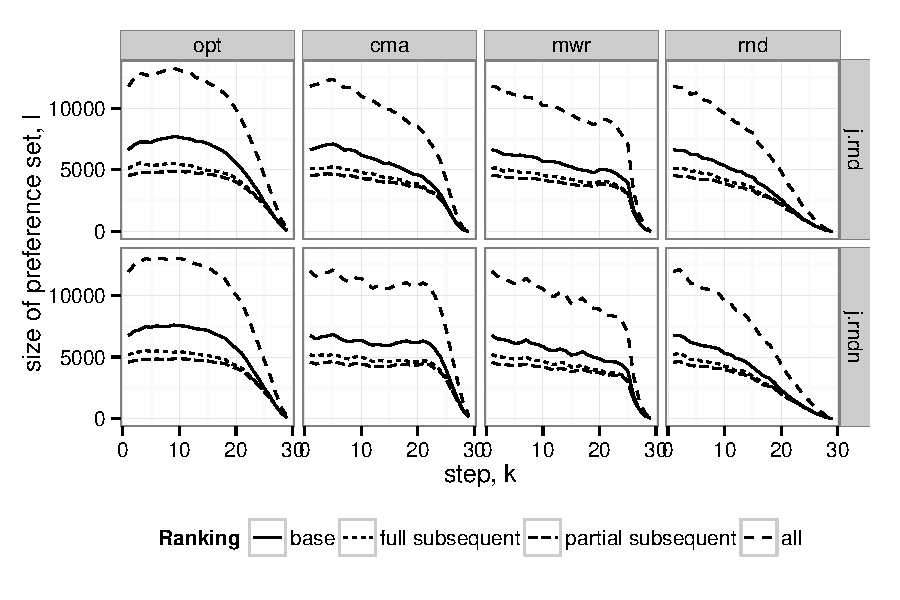
\includegraphics[width=\columnwidth]{figures/numTrainingData}
\caption{Size of preference set, $l=|S|$, for different trajectories and ranking strategies obtained from the training set for problem spaces $\mathcal{P}_{j.rnd}$ and $\mathcal{P}_{j.rndn}$.}
\label{fig:sizeofprefset}
\end{figure}


\begin{figure}[t]\centering 
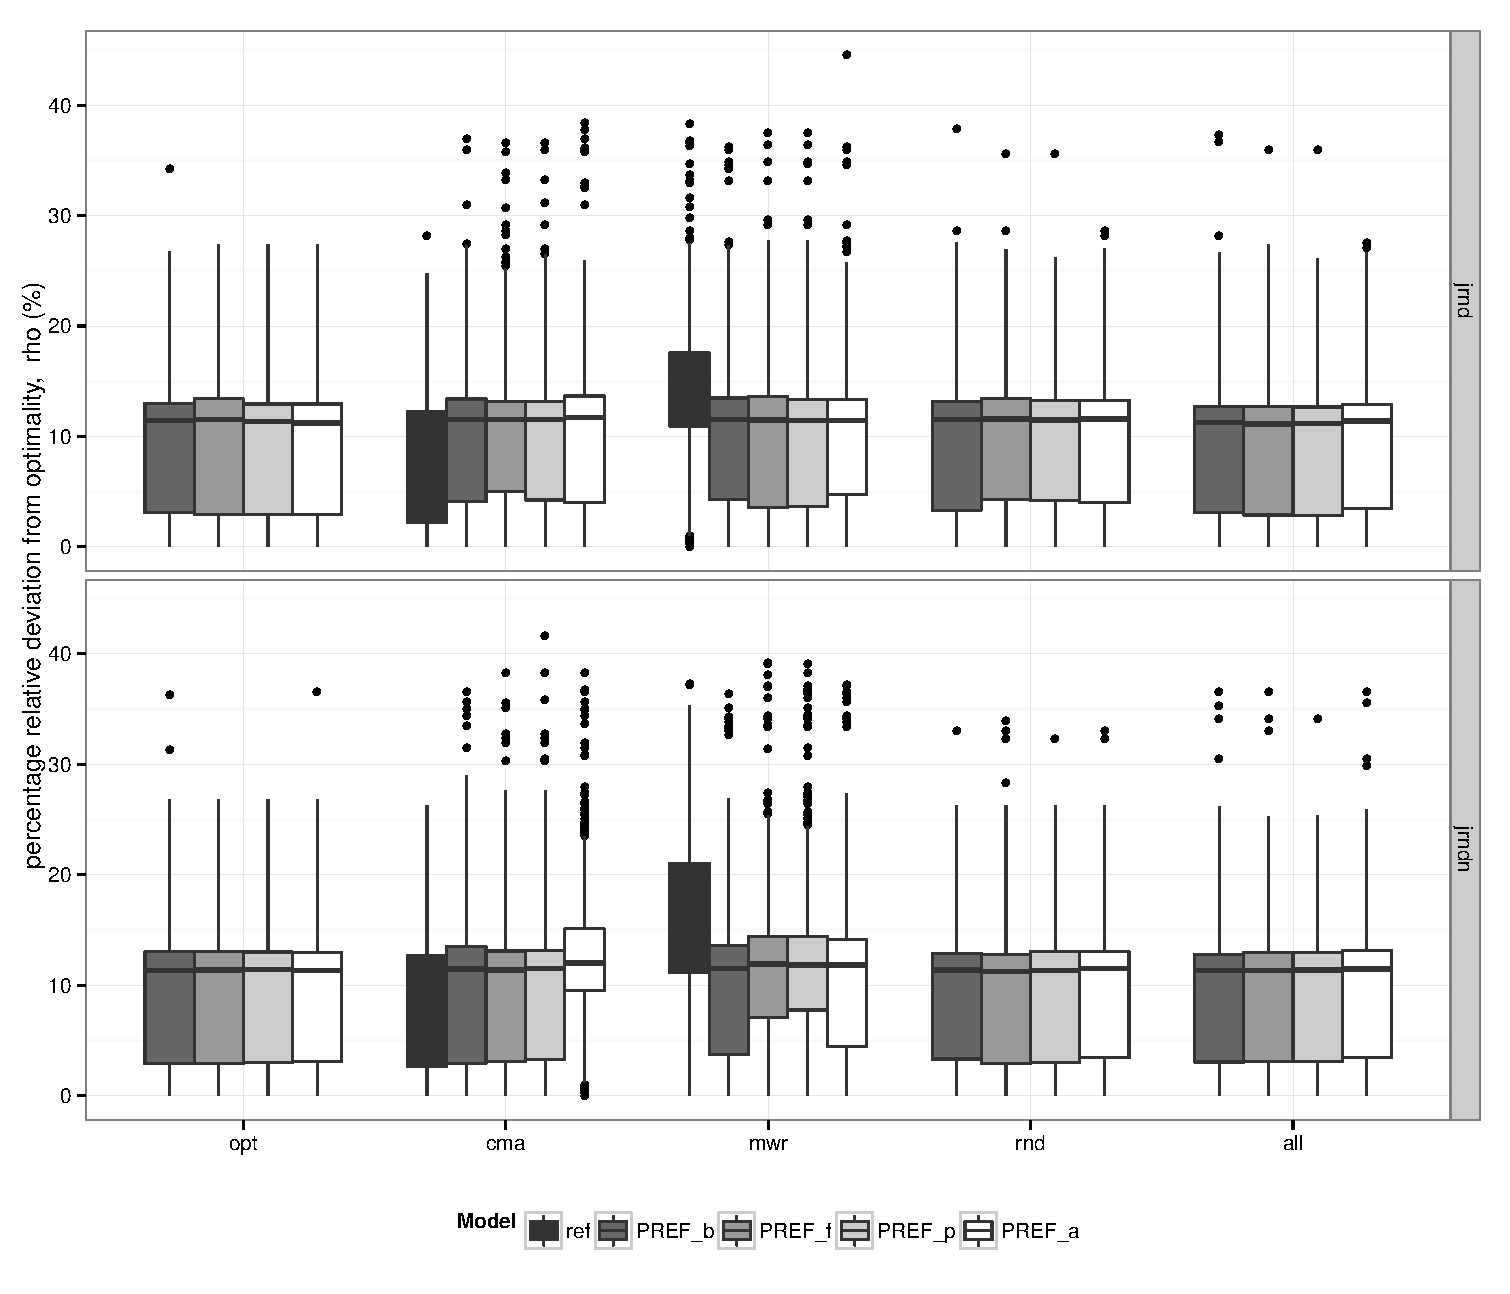
\includegraphics[width=\columnwidth]{figures/boxplot} 
\caption{Box-plot of results for linear ordinal regression model trained on various preference sets using test sets for problem spaces $\mathcal{P}_{j.rnd}$ and $\mathcal{P}_{j.rndn}$.  }
\label{fig:results}
\end{figure}
 
 
 \begin{table}[h!t] \centering
 \caption{Main statistics of percentage relative deviation from optimality, $\rho$, defined by \cref{eq:ratio} for various models.}
\label{tbl:results}
 \subfloat[][$\mathcal{P}_{ j.rnd }$ test set]{ \label{tbl:results:jrnd}
  {\scriptsize
  \begin{tabular}{rllrrrr}
    \toprule
  model&track&rank & mean & med & sd & max \\ 
    \midrule
  CMA&& & 8.84 & 10.59 & 6.14 &  28.18 \\ 
    PREF&all&p & 9.63 & 11.16 & 6.32 &  35.97 \\ 
    PREF&all&f & 9.68 & 11.11 & 6.38 &  35.97 \\ 
    PREF&opt&a & 9.92 & 11.22 & 6.49 &  27.39 \\ 
    PREF&all&b & 9.98 & 11.27 & 6.61 &  37.36 \\ 
    PREF&opt&b & 10.05 & 11.45 & 6.53 &  34.23 \\ 
    PREF&opt&p & 10.13 & 11.33 & 6.74 &  27.39 \\ 
    PREF&all&a & 10.15 & 11.38 & 6.30 &  27.57 \\ 
    PREF&opt&f & 10.31 & 11.54 & 6.87 &  27.39 \\ 
    PREF&rnd&b & 10.51 & 11.55 & 6.86 &  37.87 \\ 
    PREF&rnd&p & 10.75 & 11.49 & 6.70 &  35.60 \\ 
    PREF&cma&p & 10.78 & 11.52 & 6.89 &  36.60 \\ 
    PREF&rnd&a & 10.82 & 11.59 & 6.73 &  28.65 \\ 
    PREF&cma&f & 10.90 & 11.55 & 6.89 &  36.60 \\ 
    PREF&cma&b & 10.90 & 11.55 & 7.10 &  36.91 \\ 
    PREF&mwr&p & 10.95 & 11.46 & 7.26 &  37.47 \\ 
    PREF&mwr&f & 11.07 & 11.48 & 7.35 &  37.47 \\ 
    PREF&rnd&f & 11.09 & 11.58 & 6.92 &  35.60 \\ 
    PREF&mwr&a & 11.09 & 11.44 & 7.21 &  44.55 \\ 
    PREF&mwr&b & 11.30 & 11.54 & 7.63 &  36.26 \\ 
    PREF&cma&a & 11.39 & 11.74 & 7.59 &  38.38 \\ 
    MWR&& & 13.76 & 12.72 & 7.41 &  38.27 \\ 
     \bottomrule
  \end{tabular}
  }
 }
 \subfloat[][$\mathcal{P}_{ j.rndn }$ test set]{\label{tbl:results:jrndn}
 {\scriptsize
  \begin{tabular}{rllrrrr}
    \toprule
  model&track&rank& mean & med & sd & max \\ 
    \midrule
  CMA && & 9.13 & 10.91 & 6.16 &  26.23 \\ 
    PREF&rnd&b & 9.82 & 11.36 & 6.07 &  33.05 \\ 
    PREF&rnd&f & 9.87 & 11.22 & 6.57 &  33.92 \\ 
    PREF&opt&b & 9.94 & 11.31 & 6.52 &  36.32 \\ 
    PREF&opt&f & 9.98 & 11.36 & 6.58 &  26.84 \\ 
    PREF&rnd&p & 9.99 & 11.35 & 6.42 &  32.33 \\ 
    PREF&opt&a & 10.01 & 11.34 & 6.31 &  36.60 \\ 
    PREF&all&f & 10.05 & 11.33 & 6.53 &  36.60 \\ 
    PREF&opt&p & 10.06 & 11.42 & 6.52 &  26.84 \\ 
    PREF&all&p & 10.08 & 11.39 & 6.49 &  34.15 \\ 
    PREF&all&b & 10.12 & 11.34 & 6.73 &  36.60 \\ 
    PREF&rnd&a & 10.14 & 11.49 & 6.25 &  33.05 \\ 
    PREF&all&a & 10.39 & 11.45 & 6.69 &  36.60 \\ 
    PREF&cma&f & 10.56 & 11.38 & 7.28 &  38.31 \\ 
    PREF&cma&b & 10.73 & 11.47 & 7.62 &  36.60 \\ 
    PREF&cma&p & 10.74 & 11.51 & 7.43 &  41.60 \\ 
    PREF&mwr&b & 11.33 & 11.52 & 7.72 &  36.41 \\ 
    PREF&mwr&a & 11.70 & 11.82 & 7.88 &  37.20 \\ 
    PREF&mwr&f & 12.07 & 11.93 & 8.07 &  39.17 \\ 
    PREF&mwr&p & 12.14 & 11.84 & 8.32 &  39.12 \\ 
    PREF&cma&a & 12.59 & 12.02 & 7.94 &  38.27 \\ 
    MWR&& & 14.16 & 12.74 & 7.59 & 37.25 \\ 
     \bottomrule
  \end{tabular}
  } 
  }
 \end{table}
 
 
 
\subsection{Ranking strategies}\label{sec:expr:rank}
There is no statistical difference between \PREF{}{f} and \PREF{}{p} ranking-models across all trajectory disciplines (cf. 
Fig. \ref{fig:results}), which is expected since $S_p$ is designed to contain 
the same preference information as $S_f$. The results hold for both problem spaces. 

Combining the ranking schemes, $S_{a}$, does not improve the individual ranking-schemes as there is no statistical difference between \PREF{}{a} and \PREF{}{b}, \PREF{}{f} nor \PREF{}{p}  across all  disciplines, save \PREF{cma}{a} for $\mathcal{P}_{j.rndn}$ which yielded a considerably worse mean relative error. 

Moreover, there is no statistical difference between either of the subsequent ranking-schemes outperform and the original $S_b$ set-up from \cite{InRu11a}. However overall, the subsequent ranking schemes results in lower mean relative error, and since a smaller preference set is preferred, it is opted to use the $S_{p}$ ranking scheme. 

Furthermore, it is noted that \PREF{mwr}{} model is able to significantly outperform the original heuristics, MWR, used to create the training data $\Phi^{mwr}$, irrespective of the ranking schemes. Whereas the fixed weights found via CMA-ES outperform the \PREF{cma}{} models for all ranking schemes. This implies that ranking scheme is relatively irrelevant. The results hold for both problem spaces. 

\subsection{Trajectory sampling strategies}\label{sec:expr:track}
Learning preference pairs from a good scheduling policies, as done  in \PREF{cma}{} and \PREF{mwr}{}, can give favourable results, however tracking optimal paths yields generally a lower mean relative error. 

It is particularly interesting there is no statistical difference between \PREF{opt}{} and \PREF{rnd}{} for both 
$\mathcal{P}_{j.rnd}$ and $\mathcal{P}_{j.rndn}$ ranking-models. That is to say, tracking optimal dispatches gives the same performance as completely random dispatches. This indicates that exploring 
only optimal trajectories can result in a training set where the learning algorithm is inept to determine good 
dispatches in the circumstances when newly encountered features have diverged from the learned feature set labelled to optimum solutions. 

Finally, \PREF{all}{} and \PREF{opt}{} gave the best combination for $\mathcal{P}_{j.rnd}$ and $\mathcal{P}_{j.rndn}$, however in the latter case \PREF{rnd}{} had the best mean relative error although not statistically different from \PREF{all}{} and \PREF{opt}{}.

For $\mathcal{P}_{j.rnd}$  the best mean relative error was for \PREF{all}{}, in that case adding random suboptimal trajectories with the optimal trajectories gave the learning algorithm a greater variety of preference pairs for getting out of local minima. Therefore a general trajectory scheme would to explore both optimal with suboptimal paths.

\subsection{Following CMA-ES guided trajectory}\label{sec:expr:cmaes}
The rational for using the $\Phi^{cma}$ strategy was mostly due to the fact a linear classifier is creating the training data (using the weights found via CMA-ES optimisation), hence the training data created should be linearly separable, which in turn should boost the training accuracy for a linear classification learning model. However, this is not the case, since \PREF{cma}{} does not improve the original CMA-ES heuristic which 
was used to guide its training set $\Phi^{cma}$. However the \PREF{cma}{} approach is preferred to that of \PREF{mwr}{}, so there is some information gained by following the CMA-ES obtained weights instead of simple priority dispatching rules, such as MWR. 
%
Let's inspect the CMA-ES guided training data more closely, in particular the linear weights for \cref{eq:jssp:linweights}. The weights are depicted in \cref{fig:weights} for problem spaces $\mathcal{P}_{j.rnd}$ (left) and $\mathcal{P}_{j.rndn}$ (right). The original weights found via CMA-ES optimisation, that are used to guide the collection of training data, are depicted dashed whereas weights obtained by the linear classification \PREF{cma}{p} model are depicted solid. 

From the CMA-ES experiments it is clear that a lot of weight is applied to decision variable $w_6$, which corresponds implementing MWR, yet the existing weights for other features directs the evolutionary search to a ``better'' training data to learn, than the PREF models. Arguably, the training data could be even better, however implementing CMA-ES is rather costly, in fact in \cite{InRu14a} the optimisation had not fully converged given its allocated 288hrs of computation time.

It might also be an artefact due to the fact that the sampling of the feature space during CMA-ES search is completely different to the data generation described in this study. Hence the different scaling parameters for the features might influence the results. Moreover, the CMA-ES is minimizing the makespan directly, whereas the PREF models are learning to discriminate optimal versus suboptimal features sets that  are believed to imply a better deviation from optimality later on. However, in that case, the process is very vulnerable when it comes to any divergence from the optimal path. 
Ideally,  it would be best to combine both methodologies: Collect training data from the CMA-ES optimisation which optimises w.r.t. the ultimate performance measure used, and in order to improve upon those weights even further, use a preference based learning approach to deter from any local minima. 

\begin{figure}\centering
\subfloat[][$\mathcal{P}_{j.rnd}$]{\label{fig:weights:jrnd}
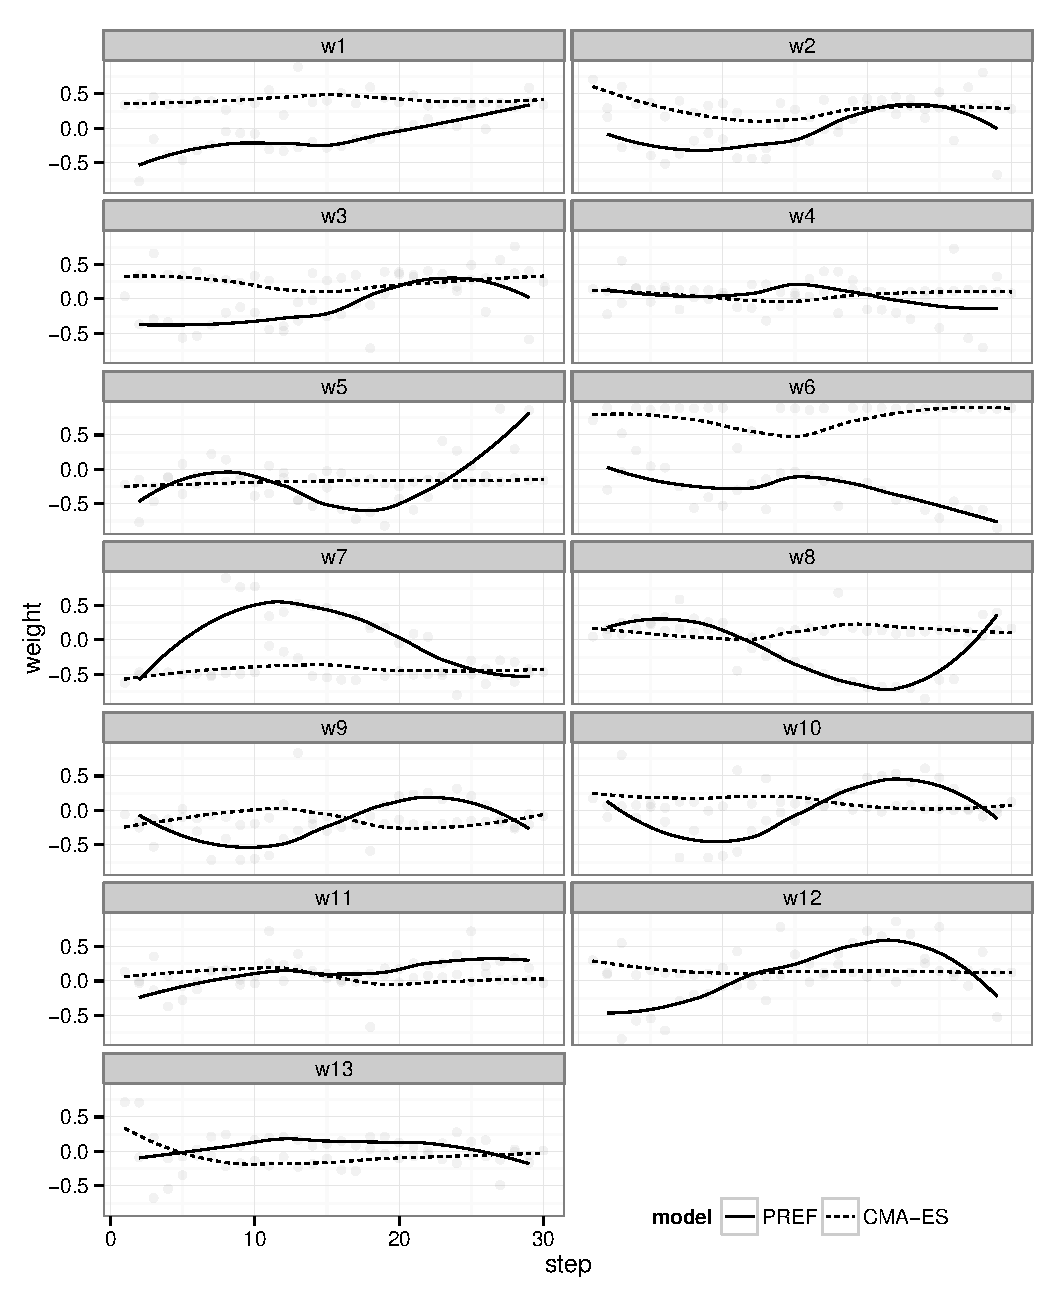
\includegraphics[width=0.47\linewidth]{figures/weights_jrnd}}
\subfloat[][$\mathcal{P}_{j.rndn}$]{\label{fig:weights:jrndn}
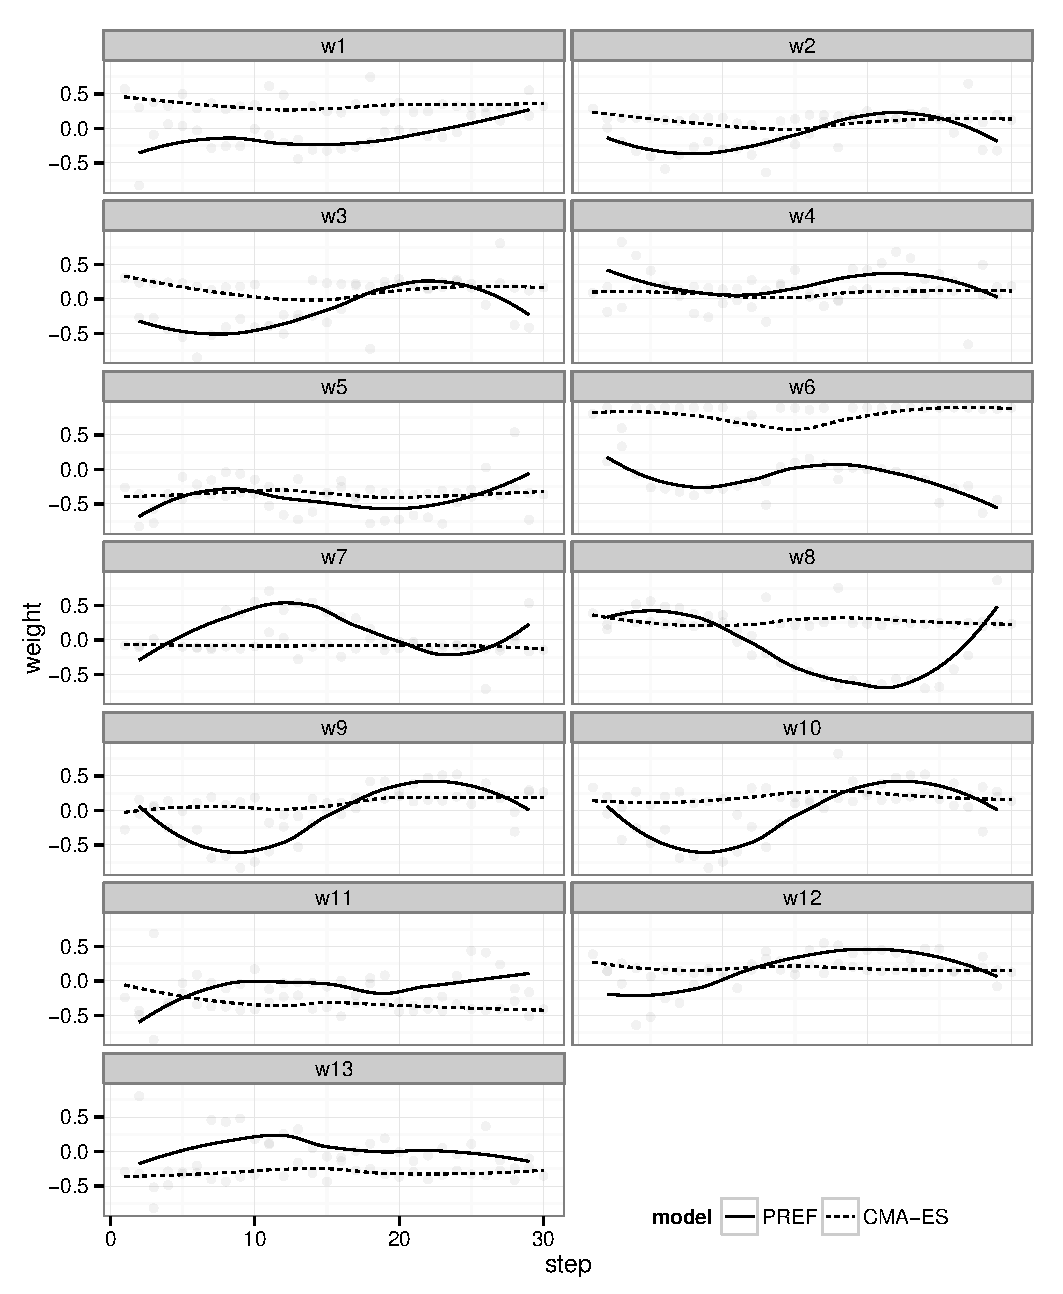
\includegraphics[width=0.47\linewidth]{figures/weights_jrndn}}
\caption{Linear weights ($w_1$ to $w_{13}$ from left to right, top to bottom) found via CMA-ES optimisation (dashed), and weights found via learning classification \PREF{cma}{p} model (solid). }\label{fig:weights}
\end{figure}

\section{Summary and conclusion}\label{sec:summary}
The study presents strategies for how to generate training data to be used in supervised learning of linear composite dispatching rules for job-shop scheduling.
The experimental results provide evidence of the benefit of adding sub-optimal solutions to the training set, apart from optimal ones.
The classification of optimal\footnote{Here the tasks labelled `optimal' do not necessarily yield the optimum makespan (except in the case of following optimal trajectories), instead these are the optimal dispatches for the given partial schedule.} and suboptimal features are of paramount importance. The subsequent rankings are not of much value, since they are disregarded anyway. 
However, the trajectories to create training instances have to be varied to boost performance. This is due to the  fact that sampling only states that  correspond  to optimal or close-to optimal schedules isn't of much use when the model has diverged too far. Since we are dealing with sequential decision making, all future observation are dependent on previous operations. 
Therefore, to account for this drawback, an imitation learning approach  by \cite{RossB10,RossGB11} could fruitful. 
In that case, we could continue with our \PREF{opt}{} model, and collect a new training set by following the learned policy and use that to create a new model similar to the $\Phi^{all}$ scheme. In short, using the model to update itself. 
This can be done several times until the weights converge. The benefit of this approach is that the states that are likely to occur in practice are investigated, and as such used to dissuade the model from making poor choices. Alas, due to the computational cost\footnote{Note, each partial schedule corresponding to a feature in $\Phi$ is optimised to obtain its correct labelling.} of collecting the training set $\Phi$, this sort of methodology isn't suitable for high dimensionality of job-shops. 

Unlike \cite{Siggi10,Malik08,Russell09} learning only optimal training data was not fruitful. However, inspired by the original work by \cite{Siggi05}, having heuristic guide the generation of training data, but with nevertheless optimal labelling based on a solver, gave meaningful preference pairs which the learning algorithm could learn. In conclusion, henceforth, the training data will be generated with \PREF{all}{p} scheme for the authors' future work.
Based on these preliminary experiments, we continue to test on a greater variety of problem data distributions for scheduling, namely job-shop and permutation flow-shop problems. Once training data has been carefully created, global dispatching rules can finally be learned, with the hope of implementing them for a greater number of jobs and machines. This is the focus of our current work.
 
 
 
\bibliography{../references}
\bibliographystyle{splncs03} 
\end{document}
